%Fred's NSF Grant Dec 2018
% GitHub: https://github.com/fjhickernell/NSF_CompMath2018Nov
% Overleaf: https://www.overleaf.com/9576964687whkhbmrrvhsd
\documentclass[11pt]{NSFamsart}
\usepackage{latexsym,amsfonts,amsmath,amsthm,epsfig,extdash,multirow}
\usepackage{stackrel,tabularx,mathtools,enumitem,xspace}
\usepackage[dvipsnames]{xcolor}
\usepackage[numbers]{natbib}
\usepackage{hyperref,accents, booktabs}
\usepackage{algorithm, algorithmicx}
\usepackage{anyfontsize}
\usepackage{cleveref}




\newcommand{\myshade}{85}
\colorlet{mylinkcolor}{violet}
\colorlet{mycitecolor}{Aquamarine}
%\colorlet{mycitecolor}{OliveGreen}
\colorlet{myurlcolor}{YellowOrange}

\hypersetup{
	linkcolor  = mylinkcolor!\myshade!black,
	citecolor  = mycitecolor!\myshade!black,
	urlcolor   = myurlcolor!\myshade!black,
	colorlinks = true,
}


% This package prints the labels in the margin
%\usepackage[notref,notcite]{showkeys}


%\pagestyle{empty}
\thispagestyle{plain}
\pagestyle{plain}

\headsep-0.6in
%\headsep-0.45in

%%list of acronyms with links
\newcommand{\QMCSoft}{\hyperlink{QMCSoftlink}{QMCSoft}\xspace}
\newcommand{\GAIL}{\hyperlink{GAILlink}{GAIL}\xspace}
\newcommand{\QMC}{\hyperlink{QMClink}{QMC}\xspace}
\newcommand{\IIDMC}{\hyperlink{IIDMClink}{IID MC}\xspace}
\newcommand{\SAMSIQMC}{\hyperlink{SAMSIlink}{SAMSI-QMC}\xspace}
\newcommand{\SciPy}{\hyperlink{SciPylink}{SciPy}\xspace}
\newcommand{\GSL}{\hyperlink{GSLlink}{GSL}\xspace}
\newcommand{\NAG}{\hyperlink{NAGlink}{NAG}\xspace}
\newcommand{\MATLAB}{\hyperlink{MATLABlink}{MATLAB}\xspace}
\newcommand{\Chebfun}{\hyperlink{Chebfunlink}{Chebfun}\xspace}
\newcommand{\Rlang}{\hyperlink{Rlink}{R}\xspace}
\newcommand{\Julia}{\hyperlink{Julialink}{Julia}\xspace}

\textwidth6.4in
\setlength{\oddsidemargin}{0in}
\setlength{\evensidemargin}{0in}
\textheight8.9in
%\textheight9.1in

\newtheorem{theorem}{theorem}


\providecommand{\FJHickernell}{Hickernell}
\newcommand{\hf}{\widehat{f}}
\newcommand{\hg}{\widehat{g}}
\newcommand{\hI}{\hat{I}}
\newcommand{\hatf}{\hat{f}}
\newcommand{\hatg}{\hat{g}}
\newcommand{\tf}{\widetilde{f}}
\newcommand{\tbf}{\tilde{\bff}}
%\DeclareMathOperator{\Pr}{\mathbb{P}}
\DeclareMathOperator{\cost}{COST}
\DeclareMathOperator{\comp}{COMP}

\DeclareMathOperator{\loss}{loss}
\DeclareMathOperator{\lof}{lof}
\DeclareMathOperator{\reg}{reg}
\DeclareMathOperator{\CV}{CV}
\DeclareMathOperator{\size}{wd}
\DeclareMathOperator{\GP}{\mathcal{G} \! \mathcal{P}}
\DeclareMathOperator{\erf}{erf}
\DeclareMathOperator*{\argmax}{arg\,max}
\DeclareMathOperator*{\argmin}{arg\,min}


\newcommand{\reals}{{\mathbb{R}}}
\newcommand{\naturals}{{\mathbb{N}}}
\newcommand{\natzero}{{\mathbb{N}_0}}
\newcommand{\integers}{{\mathbb{Z}}}
\def\expect{{\mathbb{E}}}
\def\il{\left \langle}
\def\ir{\right \rangle}
\def\e{\varepsilon}
\def\g{\gamma}
\def\l{\lambda}
\def\b{\beta}
\def\a{\alpha}
\def\lall{\Lambda^{{\rm all}}}
\def\lstd{\Lambda^{{\rm std}}}

\newcommand{\vf}{\boldsymbol{f}}
\newcommand{\hV}{\widehat{V}}
\newcommand{\tV}{\widetilde{V}}
\newcommand{\fraku}{\mathfrak{u}}
\newcommand{\hcut}{\mathfrak{h}}
\newcommand{\tOmega}{\widetilde{\Omega}}
\newcommand{\tvarrho}{\widetilde{\varrho}}

\newcommand{\bbE}{\mathbb{E}}
\newcommand{\tQ}{\widetilde{Q}}
\newcommand{\mA}{\mathsf{A}}
\newcommand{\mB}{\mathsf{B}}
\newcommand{\mC}{\mathsf{C}}
\newcommand{\mD}{\mathsf{D}}
\newcommand{\mG}{\mathsf{G}}
\newcommand{\mH}{\mathsf{H}}
\newcommand{\mI}{\mathsf{I}}
\newcommand{\bbK}{\mathbb{K}}
\newcommand{\mK}{\mathsf{K}}
\newcommand{\tmK}{\widetilde{\mathsf{K}}}
\newcommand{\mL}{\mathsf{L}}
\newcommand{\mM}{\mathsf{M}}
\newcommand{\mP}{\mathsf{P}}
\newcommand{\mQ}{\mathsf{Q}}
\newcommand{\mR}{\mathsf{R}}
\newcommand{\mX}{\mathsf{X}}
\newcommand{\mPhi}{\mathsf{\Phi}}
\newcommand{\mPsi}{\mathsf{\Psi}}
\newcommand{\mLambda}{\mathsf{\Lambda}}
\newcommand{\cube}{[0,1]^d}
\newcommand{\design}{\{\bx_i\}_{i=1}^n}

\DeclareMathOperator{\err}{err}
\DeclareMathOperator{\oerr}{\overline{\err}}
\DeclareMathOperator{\herr}{\widehat{\err}}
\DeclareMathOperator{\Ans}{ANS}

\DeclareMathOperator{\Var}{Var}
\DeclareMathOperator{\SOL}{SOL}
\DeclareMathOperator{\APP}{APP}
\DeclareMathOperator{\ALG}{ALG}
\DeclareMathOperator{\ERR}{ERR}
\DeclareMathOperator{\OPER}{OPER}



\DeclareMathOperator{\INT}{INT}
\DeclareMathOperator{\OPT}{MIN}

\newcommand{\bone}{\boldsymbol{1}}
\newcommand{\bzero}{\boldsymbol{0}}
\newcommand{\binf}{\boldsymbol{\infty}}
\newcommand{\ba}{{\boldsymbol{a}}}
\newcommand{\bb}{{\boldsymbol{b}}}
\newcommand{\bc}{{\boldsymbol{c}}}
\newcommand{\bd}{{\boldsymbol{d}}}
\newcommand{\be}{{\boldsymbol{e}}}
\newcommand{\bff}{{\boldsymbol{f}}}
\newcommand{\bhh}{{\boldsymbol{h}}}
\newcommand{\beps}{{\boldsymbol{\varepsilon}}}
\newcommand{\tbeps}{\tilde{\beps}}
\newcommand{\bx}{{\boldsymbol{x}}}
\newcommand{\bX}{{\boldsymbol{X}}}
\newcommand{\bh}{{\boldsymbol{h}}}
\newcommand{\bj}{{\boldsymbol{j}}}
\newcommand{\bk}{{\boldsymbol{k}}}
\newcommand{\bg}{{\boldsymbol{g}}}
\newcommand{\bn}{{\boldsymbol{n}}}
\newcommand{\bv}{{\boldsymbol{v}}}
\newcommand{\bu}{{\boldsymbol{u}}}
\newcommand{\by}{{\boldsymbol{y}}}
\newcommand{\bt}{{\boldsymbol{t}}}
\newcommand{\bz}{{\boldsymbol{z}}}
\newcommand{\bvarphi}{{\boldsymbol{\varphi}}}
\newcommand{\bgamma}{{\boldsymbol{\gamma}}}
\newcommand{\bphi}{{\boldsymbol{\phi}}}
\newcommand{\bpsi}{{\boldsymbol{\psi}}}
\newcommand{\bnu}{{\boldsymbol{\nu}}}
\newcommand{\balpha}{{\boldsymbol{\alpha}}}
\newcommand{\bbeta}{{\boldsymbol{\beta}}}
\newcommand{\bo}{{\boldsymbol{\omega}}}  %GF added
\newcommand{\newton}[2]{\left(\begin{array}{c} #1\\ #2\end{array}\right)}
\newcommand{\anor}[2]{\| #1\|_{\mu_{#2}}}
\newcommand{\satop}[2]{\stackrel{\scriptstyle{#1}}{\scriptstyle{#2}}}
\newcommand{\setu}{{\mathfrak{u}}}

\newcommand{\me}{\textup{e}}
\newcommand{\mi}{\textup{i}}
\def\d{\textup{d}}
\def\dif{\textup{d}}
\newcommand{\cc}{\mathcal{C}}
\newcommand{\cb}{\mathcal{B}}
\newcommand{\cl}{L}
\newcommand{\ct}{\mathfrak{T}}
\newcommand{\cx}{{\Omega}}
\newcommand{\cala}{{\mathcal{A}}}
\newcommand{\calc}{{\mathcal{C}}}
\newcommand{\calf}{{\mathcal{F}}}
\newcommand{\calfd}{{\calf_d}}
\newcommand{\calh}{{\mathcal{H}}}
\newcommand{\tcalh}{{\widetilde{\calh}}}
\newcommand{\calI}{{\mathcal{I}}}
\newcommand{\calhk}{\calh_d(K)}
\newcommand{\calg}{{\mathcal{G}}}
\newcommand{\calgd}{{\calg_d}}
\newcommand{\caln}{{\mathcal{N}}}
\newcommand{\cL}{\mathcal{L}}
\newcommand{\cP}{\mathcal{P}}
\newcommand{\cT}{\mathcal{T}}
\newcommand{\cK}{\mathcal{K}}
\newcommand{\fA}{\mathfrak{A}}
\newcommand{\fC}{\mathfrak{C}}
\newcommand{\fF}{\mathfrak{F}}
\newcommand{\fL}{\mathfrak{L}}
\newcommand{\fU}{\mathfrak{U}}
\newcommand{\hS}{\widehat{S}}
\DeclareMathOperator{\Prob}{\mathbb{P}}

\def\abs#1{\ensuremath{\left \lvert #1 \right \rvert}}
\newcommand{\bigabs}[1]{\ensuremath{\bigl \lvert #1 \bigr \rvert}}
\newcommand{\norm}[2][{}]{\ensuremath{\left \lVert #2 \right \rVert}_{#1}}
\newcommand{\ip}[3][{}]{\ensuremath{\left \langle #2, #3 \right \rangle_{#1}}}
\newcommand{\bignorm}[2][{}]{\ensuremath{\bigl \lVert #2 \bigr \rVert}_{#1}}
\newcommand{\Bignorm}[2][{}]{\ensuremath{\Bigl \lVert #2 \Bigr \rVert}_{#1}}
\newcommand{\calm}{{\mathfrak{M}}}
\DeclareMathOperator{\diag}{diag}
\DeclareMathOperator{\dist}{dist}
\DeclareMathOperator{\filldis}{fill}
\DeclareMathOperator{\sep}{sep}
\DeclareMathOperator{\avg}{avg}
\DeclareMathOperator{\vol}{vol}
\DeclareMathOperator{\cov}{cov}

\newcommand{\des}{\{\bx_i\}}
\newcommand{\desinf}{\{\bx_i\}_{i=1}^{\infty}}
\newcommand{\desn}{\{\bx_i\}_{i=1}^n}
\newcommand{\wts}{\{g_i\}_{i=1}^N}
\newcommand{\wtsn}{\{g_i\}_{i=1}^N}
\newcommand{\datan}{\{y_i\}_{i=1}^N}

%FJH added
\newcommand{\Order}{\mathcal{O}}
\newcommand{\ch}{\mathcal{H}}
\newcommand{\tch}{{\widetilde{\ch}}}
\newcommand{\veps}{\boldsymbol{\varepsilon}}
\DeclareMathOperator{\best}{best}
\newcommand{\hmu}{\hat{\mu}}
\newcommand{\hsigma}{\hat{\sigma}}
\newcommand{\tK}{\widetilde{K}}
%\newcommand{\Matlab}{{\sc Matlab}\xspace}
\newcommand{\abstol}{\varepsilon_{\text{a}}}
\newcommand{\reltol}{\varepsilon_{\text{r}}}

\newcommand\starred[1]{\accentset{\star}{#1}}

\newcommand{\designInf}{\{\bx_i\}_{i=1}^\infty}
\newcommand{\dataN}{\bigl\{\bigl(\bx_i,f(\bx_i)\bigr)\bigr\}_{i=1}^n}
\newcommand{\dataNp}{\bigl\{\bigl(\bx_i,f(\bx_i)\bigr)\bigr\}_{i=1}^{n'}}
\newcommand{\dataNo}{\bigl\{\bigl(\bx_i,f(\bx_i)\bigr)\bigr\}_{i=1}^{n_0}}
\newcommand{\ErrN}{\ERR\bigl(\dataN,n\bigr)}
\newcommand{\fint}{f_{\text{int}}}
\newcommand{\inflate}{\fC}


\definecolor{MATLABOrange}{rgb}{0.85,  0.325, 0.098}

%\newtheorem{resproblem}{Research Problem}
%\newtheorem{research}{Research Objectives}
%\newtheorem{keyidea}{Key Idea}
\newcounter{keyideabean}[section]
\newenvironment{keyidea}{\refstepcounter{keyideabean}\par \smallskip
   \noindent\begin{itshape}%
   Key Idea~\thekeyideabean.\ignorespaces}%
   {\end{itshape}\ignorespacesafterend}


%\setcounter{page}{1}
\usepackage{algpseudocode}
\algnewcommand\algorithmicparam{\textbf{Parameters:}}
\algnewcommand\PARAM{\item[\algorithmicparam]}
\algnewcommand\algorithmicinput{\textbf{Input:}}
\algnewcommand\INPUT{\item[\algorithmicinput]}
%\algnewcommand\STATE{\item}
\algnewcommand\RETURN{\State \textbf{Return }}


\setlist[description]{font=\normalfont\itshape}

\makeatletter
\newenvironment{varsubequations}[1]
 {%
  \addtocounter{equation}{-1}%
  \begin{subequations}
  \renewcommand{\theparentequation}{#1}%
  \def\@currentlabel{#1}%
 }
 {%
  \end{subequations}\ignorespacesafterend
 }
\makeatother


%\newcommand{\smallerscoop}{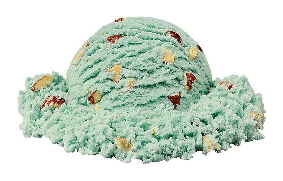
\includegraphics[width=0.7cm]{ProgramsImages/IceCreamScoop.eps}\xspace}
\newcommand{\smallerscoop}{\parbox{0.7cm}{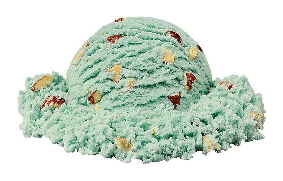
\includegraphics[width=0.7cm]{ProgramsImages/IceCreamScoop.eps}}\xspace}
\newcommand{\smallscoop}{\parbox{1cm}{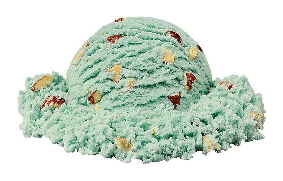
\includegraphics[width=1cm]{ProgramsImages/IceCreamScoop.eps}}\xspace}
\newcommand{\medscoop}{\parbox{1.8cm}{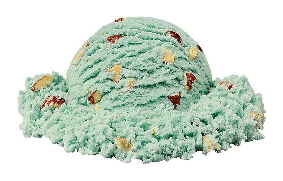
\includegraphics[width=1.8cm]{ProgramsImages/IceCreamScoop.eps}}\xspace}
\newcommand{\meddanger}{\parbox{0.8cm}{\vspace{-0.3cm}\includegraphics[width=0.75cm]{ProgramsImages/dangersign.eps}}\xspace}
\newcommand{\medcone}{\parbox{1.2cm}{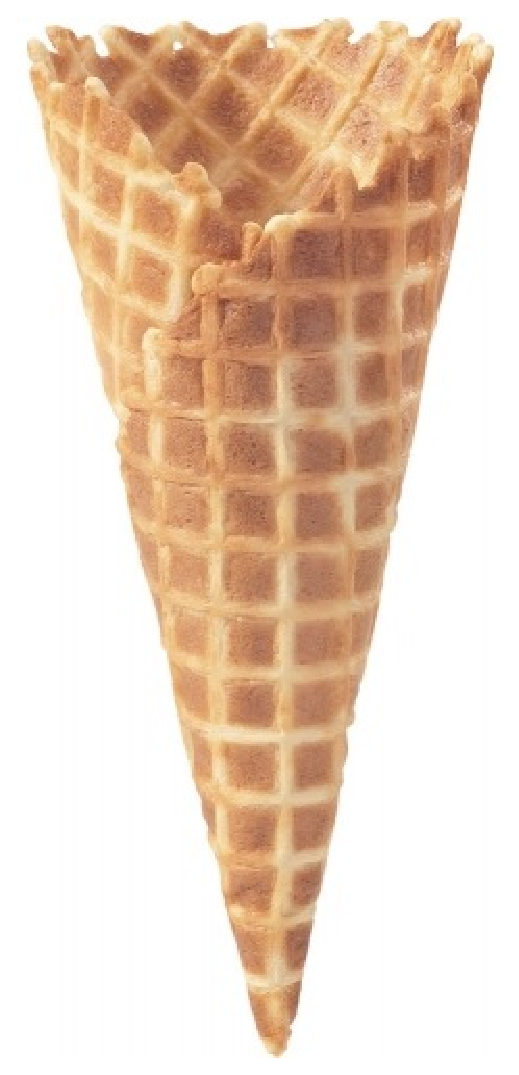
\includegraphics[width=0.55cm,angle=270]{ProgramsImages/MediumWaffleCone.eps}}\xspace}
\newcommand{\largercone}{\parbox{2.2cm}{\vspace*{-0.2cm}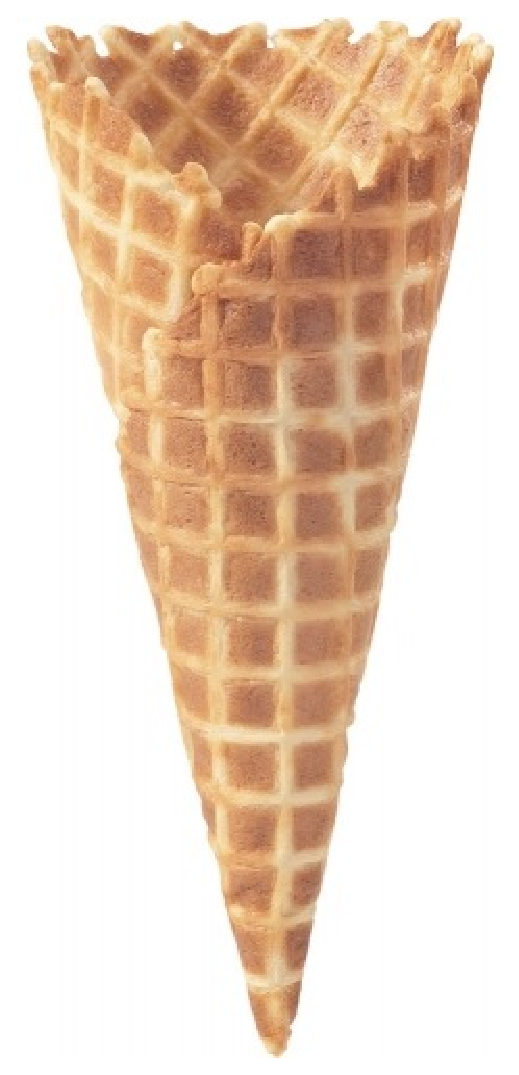
\includegraphics[width=1cm,angle=270]{ProgramsImages/MediumWaffleCone.eps}}\xspace}
\newcommand{\largecone}{\parbox{1.54cm}{\vspace*{-0.2cm}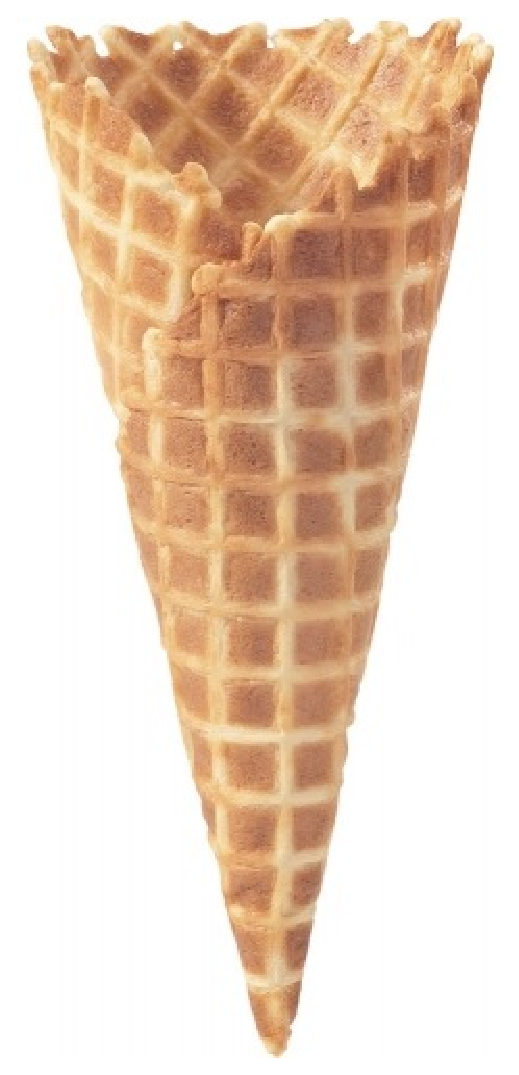
\includegraphics[width=0.7cm,angle=270]{ProgramsImages/MediumWaffleCone.eps}}\xspace}
\newcommand{\smallcone}{\parbox{0.7cm}{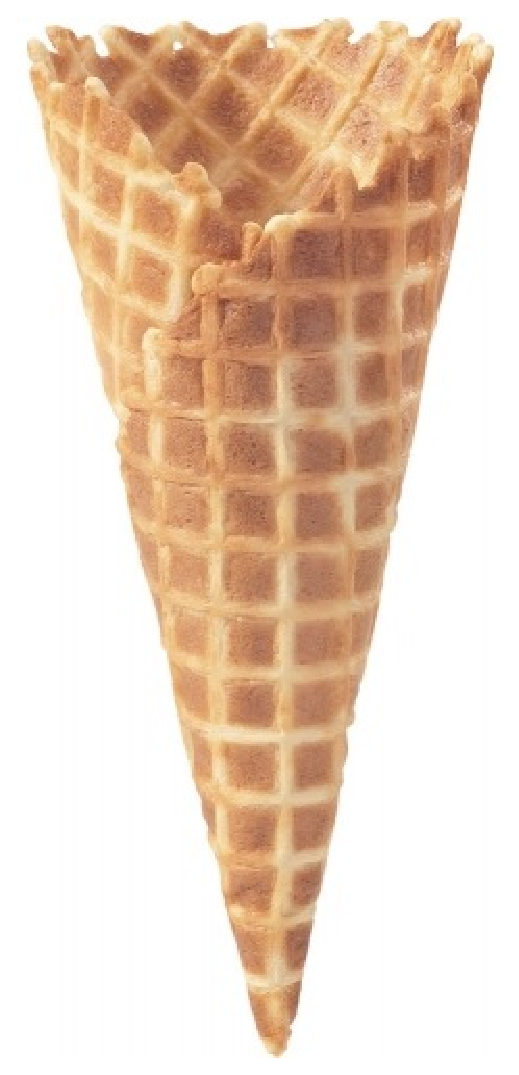
\includegraphics[width=0.32cm,angle=270]{ProgramsImages/MediumWaffleCone.eps}}\xspace}


\newcommand{\FJHNote}[1]{{\color{blue}Fred: #1}}
\newcommand{\JMHNote}[1]{{\color{green}Mac: #1}}

\newcommand{\keyideainitialtext}{The initial design must be fill the domain, $\Omega$, well enough to detect significant fluctuations in the function.}
\newcommand{\keyideafunctiontext}{The choice of the $n+1^{\text{st}}$ data site should depend meaningfully on function data, $\by_{1:n}$, not only on the location of the other sites.}
\newcommand{\keyideaBayesiantext}{Bayesian numerical analysis provides an alternative to deterministic numerical analysis.  The two perspectives produce similar outcomes.  The Bayesian perspective permits inference.}
\newcommand{\keyideaconetext}{Adaptive approximation algorithms are constructed for \emph{cones} of functions that are roughly approximated via a modest number of observations.}
\newcommand{\keyidealowdimtext}{Avoiding the curse of dimensionality requires $f$ to have an inherent low dimensional structure.}


\newcommand{\shortnoy}{For some adaptive sampling schemes, $\phi_{n+1}(\mX_{1:n},\by_{1:n}) = \phi_{n+1}(\mX_{1:n})$, meaning that these schemes are oblivious to the function values, $\by_{1:n}$.}

\newcommand{\shortheuristic}{Adaptive sampling schemes that do depend on $\by_{1:n}$ are heuristic; they lack a theoretical basis.}


\newcommand{\repeatkeyidea}[2]{\begin{itshape}Key Idea \ref{#1}. #2\end{itshape}}
\newcommand{\repeatshort}[2]{Shortcoming\ref{#1}. #2}

\begin{document}
%\setlength{\leftmargini}{2.5ex}

\begin{center}
\Large \textbf{Adaptive Sampling and Function Approximation \\ Project Description}
\end{center}
\vspace{-2ex}

\setcounter{tocdepth}{1}
\tableofcontents

\vspace{-6ex}

%%%%%%%%%%%%%%%%%%%%%%%%%%%%%%%%%%%%%%%%%%%%%%%%%%%%%%%%%%%%%%%%%%%%%%%%%%%%%%%%%%%
\section{Scientific Context, Key Ideas, and Timeliness of the Proposed Research}
%%%%%%%%%%%%%%%%%%%%%%%%%%%%%%%%%%%%%%%%%%%%%%%%%%%%%%%%%%%%%%%%%%%%%%%%%%%%%%%%%%%
Surrogate models are approximations to functions, $f: \Omega \subseteq \reals^d \to \reals$, that are very expensive to evaluate.  An example $f$ is the output of a complex time-consuming computer simulation.  Accurate surrogate models require a well-chosen design, $\mX_{1:n} := (\bx_1, \ldots, \bx_n)^T \in \Omega^{n} \subseteq \reals^{n \times d}$, i.e., an array of data sites where $f$ is to be evaluated.  Ideally, the choice of the design should be \emph{adaptive} to be optimally efficient.  The sampled function values should inform the choice of the \emph{next} data site: 
\begin{equation} \label{adaptsite}
    \bx_{n+1} = \phi_{n+1}(\mX_{1:n},\by_{1:n}), \quad \by_{1:n} := (f(\bx_1), \ldots, f(\bx_n))^T, \qquad n \in \naturals,
\end{equation}
where $\phi_{n+1} : \Omega^{n} \times \reals^n \to \Omega$ is some well chosen function that depends on underlying assumptions about $f$.  If $f$ is detected to be highly variable in one portion of the domain, $\Omega$, then more data sites should be placed there. 

Adaptive sampling and adaptive numerical algorithms are founded on the assumption that \emph{what you have not yet observed about $f$ is not much worse than what you have already observed}.  This idea must be made mathematically precise to justify any adaptive scheme.  Although adaptive sampling has been studied for decades, there remain two major shortcomings of existing theory:
\begin{enumerate}[widest = Shortcomingj, leftmargin =*]
\renewcommand{\labelenumi}{Shortcoming \arabic{enumi}.}
    \item \shortnoy \label{shortcomenoy}
    
    \item \shortheuristic
    
\end{enumerate}
\emph{The PIs, Fred J Hickernell (FJH) and Mac Hyman (MH), propose to develop theoretically sound adaptive algorithms for function approximation, which adaptively choose the data sites, as in \eqref{adaptsite}.  These adaptive algorithms will stop when the data-driven error bounds are no greater than the prescribed error tolerance.}

Several key ideas arise in the proposed research.  We list them here, illustrate them by example in this section, and then refer to them later in the proposal.
\begin{keyidea}\label{keyideainitial} \keyideainitialtext \end{keyidea}
\begin{keyidea}\label{keyideafunction} \keyideafunctiontext \end{keyidea}
\begin{keyidea}\label{keyideaBayesian} \keyideaBayesiantext \end{keyidea} 
\begin{keyidea} \label{keyideacone} \keyideaconetext \end{keyidea}
\begin{keyidea} \label{keyidealowdim} \keyidealowdimtext \end{keyidea} 


%%%%%%%%%%%%%%%%%%%%%%%%%%%%%%%%%%%%%%%%%%%%%%%%%%%%%%%%%%%%%%%%%%%%%%%%%%%%%%%%%%%
\subsection{Illustrative Univariate Example} \label{sec:UniEx}
%%%%%%%%%%%%%%%%%%%%%%%%%%%%%%%%%%%%%%%%%%%%%%%%%%%%%%%%%%%%%%%%%%%%%%%%%%%%%%%%%%%

The univariate function $f: x \mapsto \exp(-10x) \sin(8x)$, plotted in Fig.\ \ref{fig:sampleFun}, illustrates some of the challenges of adaptive sampling.  Using the $n=10$ point design, $\mX_{1:n} = (0, 0.1, \ldots, 0.6, 0.8, 0.9, 1)^T$, an approximation, $\APP(f,n)$, is constructed as the minimum norm interpolant in the Hilbert space, $\calf$, defined by its Mat\'ern reproducing kernel,
\begin{equation} \label{MatKer}
    K(t,x) = (1 + \theta \abs{t-x}) \exp(-\theta\abs{t-x}),
\end{equation}
with $\theta = 1$.  See \cite{Buh00, Fas07a, FasMcC15a, ForFly15a, ForEtal09, SchWen06a, Wen05a} for an explanation of optimal function approximation in reproducing kernel Hilbert spaces.  The approximation is given in general by
\begin{equation} \label{appxExOne}
    \APP(f,n) = \sum_{i=1}^n c_i K(\cdot, x_i), \quad \text{where } \bc = \mK^{-1} \by_{1:n}, \quad \mK = \mK(\mX_{1:n}) = \bigl( K(x_i,x_j) \bigr)_{i,j=1}^n.
\end{equation}
Fig.\ \ref{fig:sampleFun} also shows $\APP(f,10)$.  

\repeatkeyidea{keyideainitial}{\keyideainitialtext}
Here, $\APP(f,10)$ captures the peak on the left because the data sites are dense enough there.  If the design consists only of the $n=4$ sparse data sites, $\mX_{1:n} = (0, 0.4,  0.6, 1)^T$, then $\APP(f,4)$ misses the peak, as shown in Fig.\ \ref{fig:sampleFun}.  There is a substantial literature on $d$-dimensional space filling designs \cite{FangEtal19a, Jos16a, SanWilNot03}. The number of data sites required for the initial design depends on i) how many one can afford, ii) how narrow a peak one is willing to miss, and iii) the number of independent variables, $d$.

\begin{figure}[H]
    \centering
    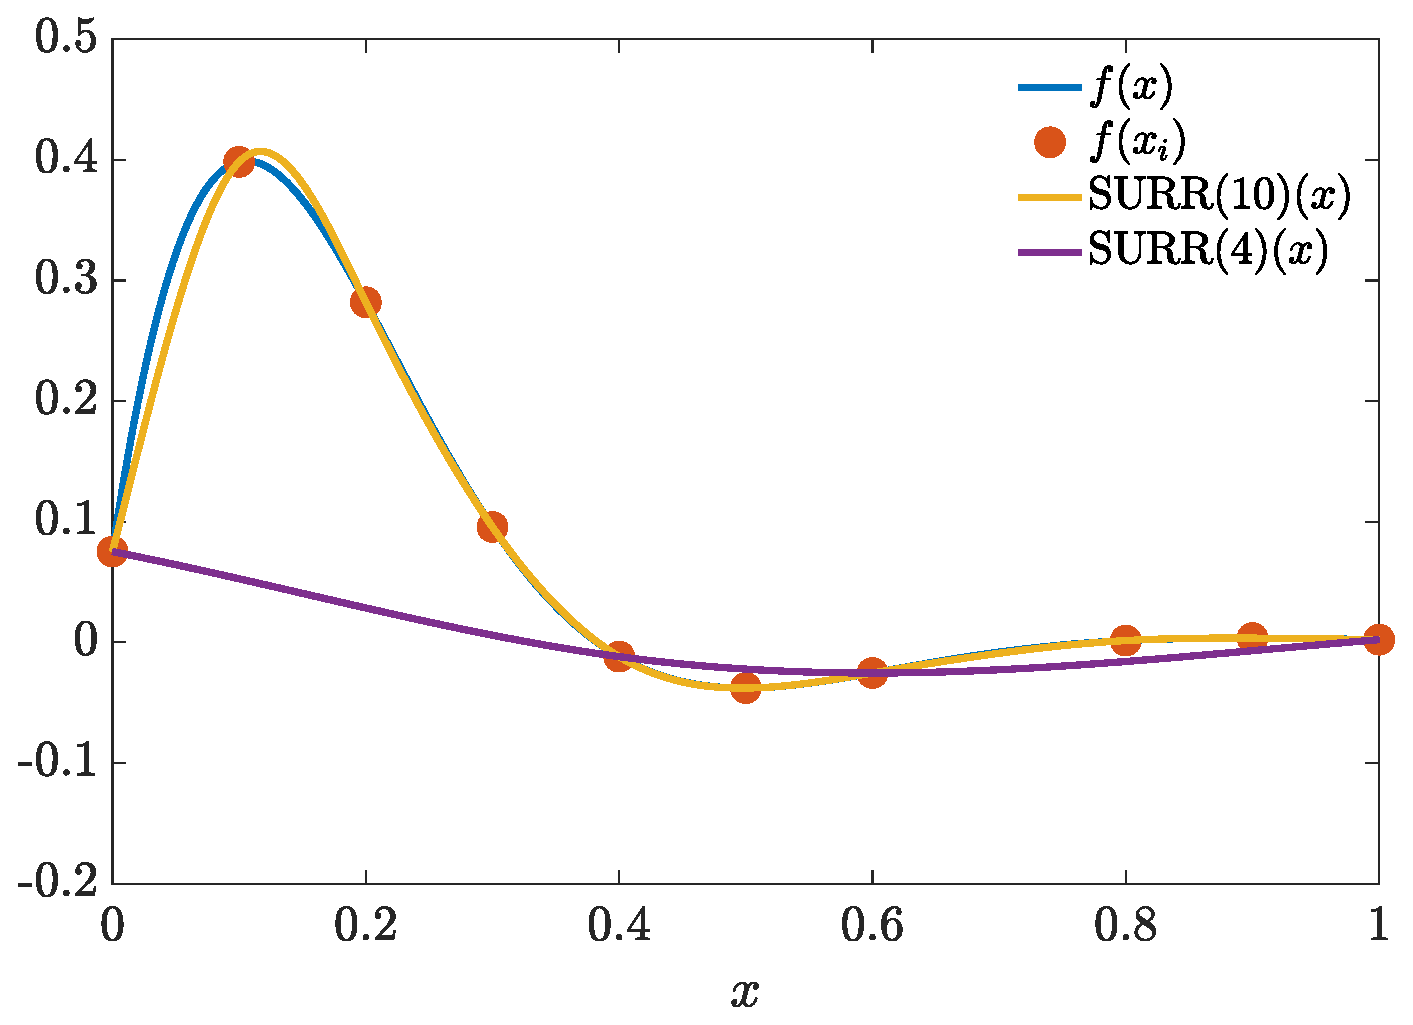
\includegraphics[width = 7cm]{ProgramsImages/fandDataAndAppxSmall.eps} \qquad \qquad
    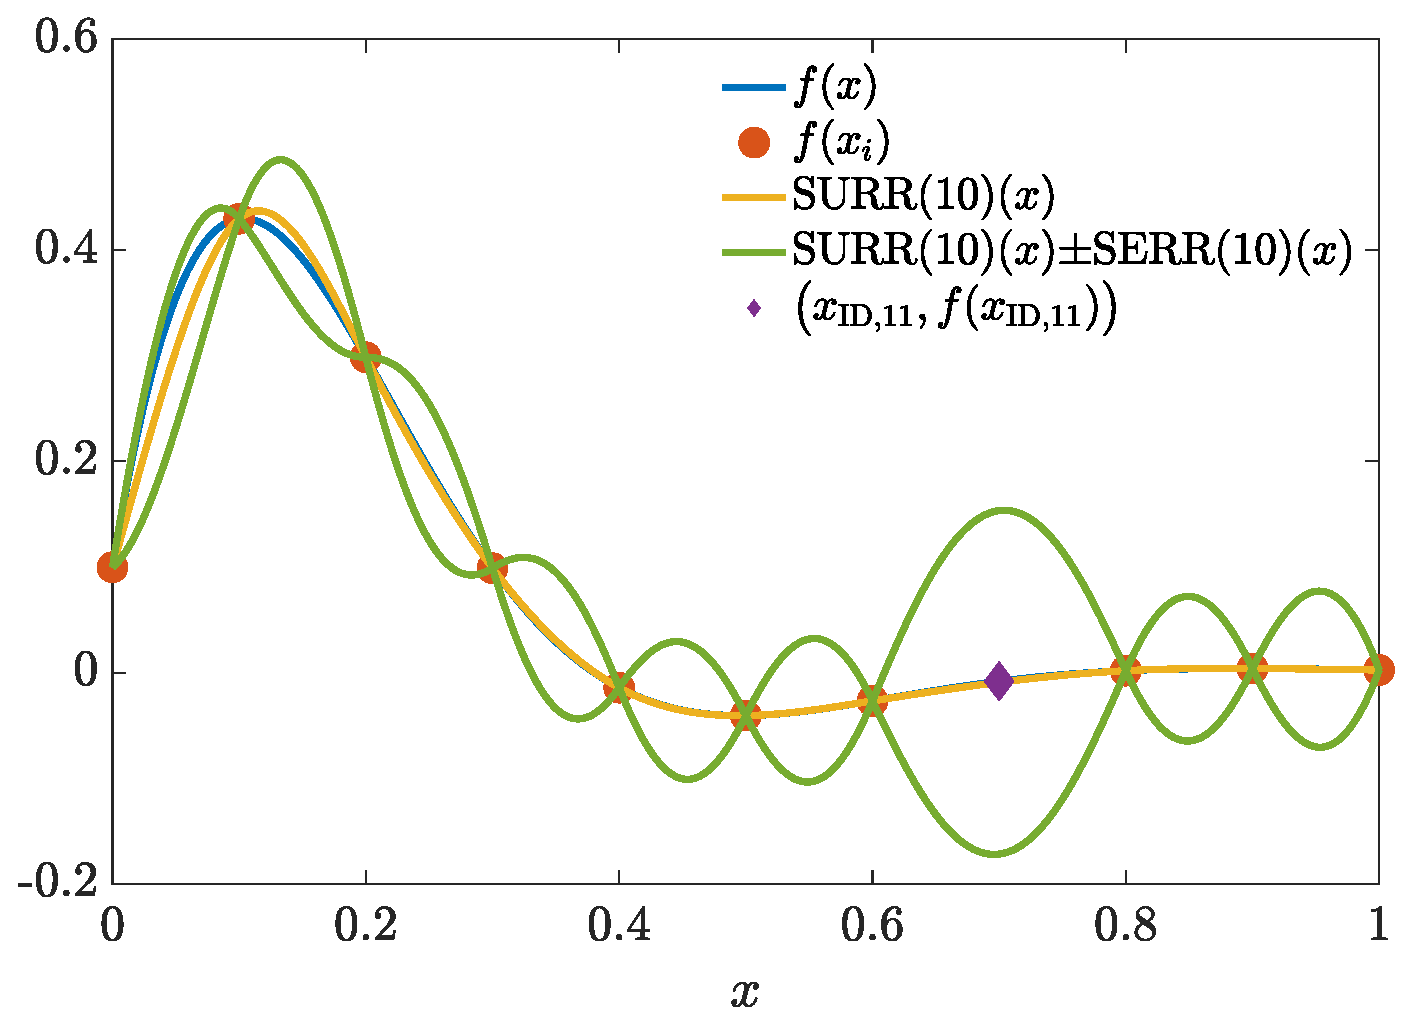
\includegraphics[width = 7cm]{ProgramsImages/fandDataAndAppxAndRMSPE.eps}
    \caption{The left plot shows $f: x \mapsto \exp(-10x) \sin(8x)$ and its approximation \eqref{appxExOne} for using $10$ and $4$ data sites and the kernel \eqref{MatKer} with $\theta = 1$. A poor approximation results from too few data sites.  The right plot includes an approximate prediction error bound, $\ERR(10,x)$ from \eqref{DataErrBda} with $A_{10} =1$, and the location of the largest prediction error, $x_{\textup{bad}}$. The largest actual error actually occurs far away from $x_{\textup{bad}}$.}
    \label{fig:sampleFun}
\end{figure}

Not surprisingly, the actual approximation error is greatest on the left side of $[0,1]$, where $f$ fluctuates the most.  Intuitively, one might expect that adding the next data site in the design on the left would yield the greatest improvement.  Unfortunately, typical adaptive schemes do not necessarily work this way (Shortcoming \ref{shortcomenoy}).

One common adaptive sampling rule is to place the next data site where the theoretical approximation error bound is maximized.  For this $\APP(f)$, the error has the following upper bound:
\begin{align}
\label{RKHSErrBd}
    \abs{f(x) - \APP(f,n)(x)} & \le \sqrt{K(x,x) - \bk^T(x) \mK^{-1} \bk(x)} \, \norm[\calf]{f - \APP(f,n)} \\
    \nonumber
    & \le \sqrt{K(x,x) - \bk^T(x) \mK^{-1} \bk(x)} \, \norm[\calf]{f},
    \quad \text{where }  \bk(x) = \bigl(K(x,x_i) \bigr)_{i=1}^n.
\end{align}
Choosing the next data site where the approximation error bound is maximized corresponds to 
\begin{equation} \label{minprederr}
    x_{n+1} = x_{\textup{bad}} = \argmax_x K(x,x) - \bk^T(x) \mK^{-1} \bk(x) = \phi_{n+1}(\mX_{1:n}),
\end{equation}
which is plotted on the right in Fig.\ \ref{fig:sampleFun}.  Since the $f(x_{\textup{bad}}) \approx \APP(f,n)(x_{\textup{bad}})$, adding $x_{\textup{bad}}$ to the design does not help much.

\repeatkeyidea{keyideafunction}{\keyideafunctiontext}
The adaptive sampling criterion in \eqref{minprederr} does not depend at all on the function data, $\by_{1:n}$, which is why it performs poorly.  For the example in Fig.\ \ref{fig:sampleFun}, a good adaptive sampling algorithm would choose the next data site on the left where it will improve upon $\APP(f,n)$ the most.  One approach to construct a good adaptive sampling criterion is to have the reproducing kernel, $K$, inferred from the function data, $\by_{1:n}$, in a significant way.  Another approach is to compute the approximation error bound only on the basis of nearby function data.  These approaches are elaborated in ???

An alternative perspective to assuming that the function to be approximated is a deterministic object in a Hilbert or Banach space is to assume that $f$ is an instance of $\GP(0,K)$, a Gaussian process with mean zero and covariance kernel, $K$.  This perspective, called Bayesian or average case numerical analysis was promoted by Diaconis \cite{Dia88a} and pursued by many others \cite{BriEtal18a, OHa91a, OwhEtal19a, RasWil06a, Rit00a}.  It assumes that $f$ is an instance of $\GP(0,K)$, a Gaussian process with mean zero and covariance kernel, $K$.  In this case the posterior mean of $f(x)$ given the data has the same expression as $\APP(f,n)$ as in \eqref{appxExOne}.

\repeatkeyidea{keyideaBayesian}{\keyideaBayesiantext}
In ??? we appeal to the Bayesian perspective.

As it stands, approximation error bound \eqref{RKHSErrBd} cannot be used as a stopping criterion for an adaptive function approximation algorithm because $\norm[\calf]{f - \APP(f,n)}$ is typically unknown.  However, if $n$ is large enough, we might hypothesize that our $f$ belongs to the cone of functions,
\begin{equation} \label{RKHScone}
    \calc := \{f \in \calf : \norm[\calf]{f - \APP(f,n)} \le A_n \norm[\calf]{\APP(f,n)} \},
\end{equation}
where $A_n$ is positive, and fixed in advance.  This $\calc$ is a cone because if $f \in \calc$, then $af \in \calc$ for any real $a$.  This $\calc$ may be interpreted as the functions in $\calf$ whose norms are not too badly approximated by $\APP(\cdot,n)$.  Since the approximation error is perpendicular to the approximation in the Hilbert space $\calf$, one may equivalently define $\calc$ as  $\{f \in \calf : \norm[\calf]{f}^2 \le (1 + A_n^2) \norm[\calf]{\APP(f,n)}^2 \}$.  Noting that $\norm[\calf]{\APP(f,n)} = \sqrt{\by_{1:n} \mK^{-1} \by_{1:n}}$ error bound \eqref{RKHSErrBd} then implies an error bound that depends completely on function data: 
\begin{subequations} \label{DataErrBd}
\begin{gather}
    \label{DataErrBda} 
    \ERR(f,n,x) : = A_n \sqrt{[K(x,x) - \bk^T(x) \mK^{-1} \bk(x)] \, [\by_{1:n}^T \mK^{-1} \by_{1:n}] }, \\
    \norm[\infty]{f - \APP(f,n)} \le \norm[\infty]{\ERR(f,n,\cdot)} \qquad \forall f \in \calc.
\end{gather}
\end{subequations}
Given method for choosing data sites adaptively, an adaptive function approximation algorithm proceeds by increasing $n$ until the right hand side of \eqref{DataErrBd} does not exceed the prescribed error tolerance, $\varepsilon$.  Then the algorithm returns $\APP(f)$.

\repeatkeyidea{keyideacone}{\keyideaconetext}
The intuition is \emph{what you cannot see is not much worse than what you can see}. All adaptive algorithms are based on this assumption.  The definition of the cone in \eqref{RKHScone} is a way of formalizing this key idea.

The cone in  \eqref{RKHScone} and the error bound in \eqref{DataErrBd} have their shortcomings. The interval $\APP(f,10)(x) \pm \ERR(f,10,x)$ does not quite cover $f(x)$ in Fig.\ 1 near $x=0$.  Part of the reason is that the kernel $K$ chosen in \eqref{MatKer} and/or the value $\theta =1$ may not be the best suited to this particular $f$.  This again raises the importance of Key Idea \ref{keyideafunction}. Also, the cone $\calc$ defined in  \eqref{RKHScone} depends strongly on the specific design chosen.  We would rather that it did not.  This point is addressed in ??.

%%%%%%%%%%%%%%%%%%%%%%%%%%%%%%%%%%%%%%%%%%%%%%%%%%%%%%%%%%%%%%%%%%%%%%%%%%%%%%%%%%%
\subsection{An Illustrative Multivariate Example} \label{ex:multi}
%%%%%%%%%%%%%%%%%%%%%%%%%%%%%%%%%%%%%%%%%%%%%%%%%%%%%%%%%%%%%%%%%%%%%%%%%%%%%%%%%%%
Although many of our key ideas can be illustrated by univariate function approximation, one key idea only makes sense in a multivariate setting.  
Let $\calf$, be the finite dimensional Banach space of multi-linear functions:
\begin{subequations} \label{ex:multilin}
\begin{gather}
    \calf = \left\{f:[0,1]^d \to \reals : f = \sum_{\bk \in \{0,1\}^d} \hf(\bk) u_{\bk} \right \}, 
    \\ 
    u_{\bk} := \prod_{k_\ell =1 }x_\ell, \quad 
    \norm[\calf]{f} : = \Bignorm[1]{\bigl(\hf(\bk)/\lambda_\bk\bigr)_{\bk \in \{0,1\}^d}},  \quad \norm[\calg]{f} : = \norm[1]{\bigl(\hf(\bk))_{\bk \in \{0,1\}^d}},
\end{gather}
\end{subequations}
for some prescribed set of weights, $(\lambda_\bk)_{\bk \in \{0,1\}^d}$, whose ordering, $\lambda_{\bk_1} \ge \lambda_{\bk_2} \ge \cdots \ge \lambda_{\bk_{2^d}}$, implies an ordering of the $\bk$.  For the sake of simplicity, suppose that you are able to sample the coefficients, $\hf(\bk)$.  In this case, the optimal approximation in the $\calg$-norm is $\APP(f,n) = \sum_{i=1}^n \hf(\bk_i) \bx_{\bk_i}$, and the error of this approximation is 
\begin{equation}
    \norm[\calg]{f - \APP(f,n)} = \norm[1]{\bigl(\hf(\bk_i) \bigr)_{i=n+1}^\infty} \le \lambda_{\bk_{n+1}} \norm[\calf]{f - \APP(f,n)} \le \lambda_{\bk_{n+1}} \norm[\calf]{f}.
\end{equation}

\repeatkeyidea{keyidealowdim}{\keyidealowdimtext}
If the $\lambda_\bk$ are all unity, then all multilinear terms are equally important according to the definition of the $\calf$-norm, and a function with unit $\calf$-norm may require $2^d$ data to ensure that the error is less than $1$.  This requirement explodes exponentially with increasing $d$.  However, if not all coordinates are equally important, and multilinear terms involving several coordinates are even less important, e.g., $\lambda_{\bk} = \prod_{k_\ell =1} w_\ell$, with the coordinate weights, $w_\ell$, decaying quickly enough, then it can be shown that $\lambda_{\bk_{n+1}}$ decays with $n$ and the curse of dimensionality is overcome \cite{DinEtal20a}.  This idea is elaborated in Sect.\ ???

%%%%%%%%%%%%%%%%%%%%%%%%%%%%%%%%%%%%%%%%%%%%%%%%%%%%%%%%%%%%%%%%%%%%%%%%%%%%%%%%%%%
\section{Results of Previous NSF-Funded Research,
NSF-DMS-1522687\except{toc}{, \\ \emph{Stable, Efficient, Adaptive Algorithms for 
Approximation and 
Integration}, \\
\$270,000, August 2015 -- July 2018}} \label{sec:Previous}
%%%%%%%%%%%%%%%%%%%%%%%%%%%%%%%%%%%%%%%%%%%%%%%%%%%%%%%%%%%%%%%%%%%%%%%%%%%%%%%%%%%

Gregory E.\ Fasshauer (GEF, co-PI) and FJH (PI) led this project, and Sou-Cheng Terrya Choi (SCTC) contributed as senior personnel.  Other major contributors were FJH's research students Yuhan Ding (YD, PhD 2015), Lan Jiang (LJ, PhD 2016), 
Llu\'is Antoni Jim\'enez Rugama (LlAJR, PhD 2016), Da Li (DL, MS 2016), Jiazhen Liu (JL, MS 2018), Jagadeeswaran Rathinavel (JR, 
PhD student), Xin Tong (XT, MS 2014, PhD student, University of Illinois at Chicago), Kan Zhang (KZ, PhD student), Yizhi Zhang (YZ, PhD 2018), and Xuan Zhou (XZ, PhD 2015).  Articles, theses,  
software, and preprints supported in 
part by this 
grant 
include 
\cite{ala_augmented_2017, 
	ChoEtal17a,
	ChoEtal17b,
	Din15a, 
	DinHic20a,
	GilEtal16a,
	Hic17a,
	HicJag18b,
	HicJim16a,
	HicEtal18a,
	HicEtal17a,
	HicKriWoz19a,
	RatHic19a,
	GilJim16b,
	JimHic16a,
	JohFasHic18a,
	Li16a,
	Liu17a,
	MarEtal18a,
	mccourt_stable_2017,
	MCCEtal19a,
	mishra_hybrid_2018,
	MisEtal19a,
	rashidinia_stable_2016,
	rashidinia_stable_2018,
	Zha18a,
	Zha17a,
	Zho15a,
	ZhoHic15a}.

%%%%%%%%%%%%%%%%%%%%%%%%%%%%%%%%%%%%%%%%%%%%%%%%%%%%%%%%%%%%%%%%%%%%%%%%%%%%%%%%%%%
\subsection{Intellectual Merit from Previous NSF Funding}
\label{previousmeritsubsec}
%%%%%%%%%%%%%%%%%%%%%%%%%%%%%%%%%%%%%%%%%%%%%%%%%%%%%%%%%%%%%%%%%%%%%%%%%%%%%%%%%%%

%%%%%%%%%%%%%%%%%%%%%%%%%%%%%%%%%%%%%%%%%%%%%%%%%%%%%%%%%%%%%%%%%%%%%%%%%%%%%%%%%%%
\subsubsection{Adaptive Algorithms for Univariate Problems} \label{sec:localadpat}
%%%%%%%%%%%%%%%%%%%%%%%%%%%%%%%%%%%%%%%%%%%%%%%%%%%%%%%%%%%%%%%%%%%%%%%%%%%%%%%%%%%
FJH, STSC, YD, XT, YZ and collaborators developed several adaptive algorithms for univariate integration, function approximation, and optimization \cite{ChoEtal17a,HicEtal14b,  Din15a, Ton14a, Zha18a}.  Most of these algorithms are \emph{globally adaptive}---the sampling density is constant (equally spaced data sites), but the number of data sites is chosen adaptively to meet the error tolerance.

However, the function approximation and integration algorithms constructed by FJH, SCTC, YD, and XT in \cite{ChoEtal17a} are \emph{locally adaptive}, meaning that the sampling density is non-uniform and influenced by the function data (Key Idea \ref{keyideafunction}).  Qualitatively, cone of functions for which these algorithms are guaranteed to succeed (Key Idea \ref{keyideacone}) consists of functions where the maximum of the second derivative in a sub-interval is not drastically smaller than it's minimum value to either the immediate left or right.  For function approximation, the adaptive sample is denser where $\abs{f''}$ is larger, as shown in Fig.\ \ref{localadaptfig}.  This locally adaptive function approximation algorithm has a computational cost of $\Order\left(\sqrt{\norm[1/2]{f''}/\varepsilon} \right)$, where $\varepsilon$ is the error tolerance, and is essentially optimal.  An intriguing aspect is the appearance of the $1/2$-quasinorm $\norm[1/2]{f''}$, which may be much smaller than 
$\norm[\infty]{f''}$ for peaky functions.

\begin{figure}[h]
	\centering
	\vspace{-1ex}
	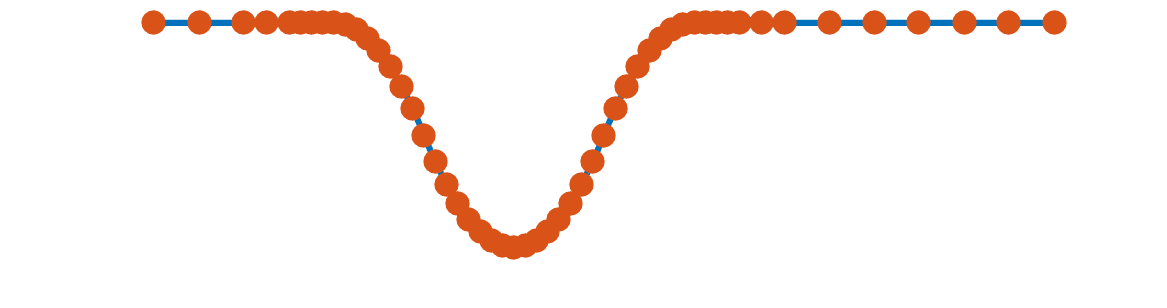
\includegraphics[width = 0.48\textwidth]{ProgramsImages/sampling-funappxg.png}

	\vspace{-2ex}
	\caption{The function data ({\color{MATLABOrange}$\bullet$}) for the locally adaptive 
	function approximation in \cite{ChoEtal17a}.  The sample is denser where $\abs{f''}$ is larger. \label{localadaptfig}}
\end{figure}

%%%%%%%%%%%%%%%%%%%%%%%%%%%%%%%%%%%%%%%%%%%%%%%%%%%%%%%%%%%%%%%%%%%%%%%%%%%%%%%%%%%
\subsubsection[QMCsec]{Globally Adaptive Cubature Based on Space-Filling Designs} \hypertarget{QMClink}{}
\label{sec:QMC}
%%%%%%%%%%%%%%%%%%%%%%%%%%%%%%%%%%%%%%%%%%%%%%%%%%%%%%%%%%%%%%%%%%%%%%%%%%%%%%%%%%%
FJH, LlAJR, DL, and JR developed globally adaptive algorithms for approximating $d$-dimensional integrals,  $\int_{[0,1]^d} f(\bx) \, \dif \bx$, based on space-filling designs \cite{HicJim16a,HicEtal17a,JimHic16a}.  Two common space-filling or low discrepancy designs are integration lattice nodes and digital sequences \cite{DicEtal14a}.  Fig.\ \ref{PtsFig} contrasts these two designs with independent and identically distributed (IID) data sites, which are not so space-filling.

\begin{figure}[h] % MATLAB Driver: PlotPoints.m
	\centering
	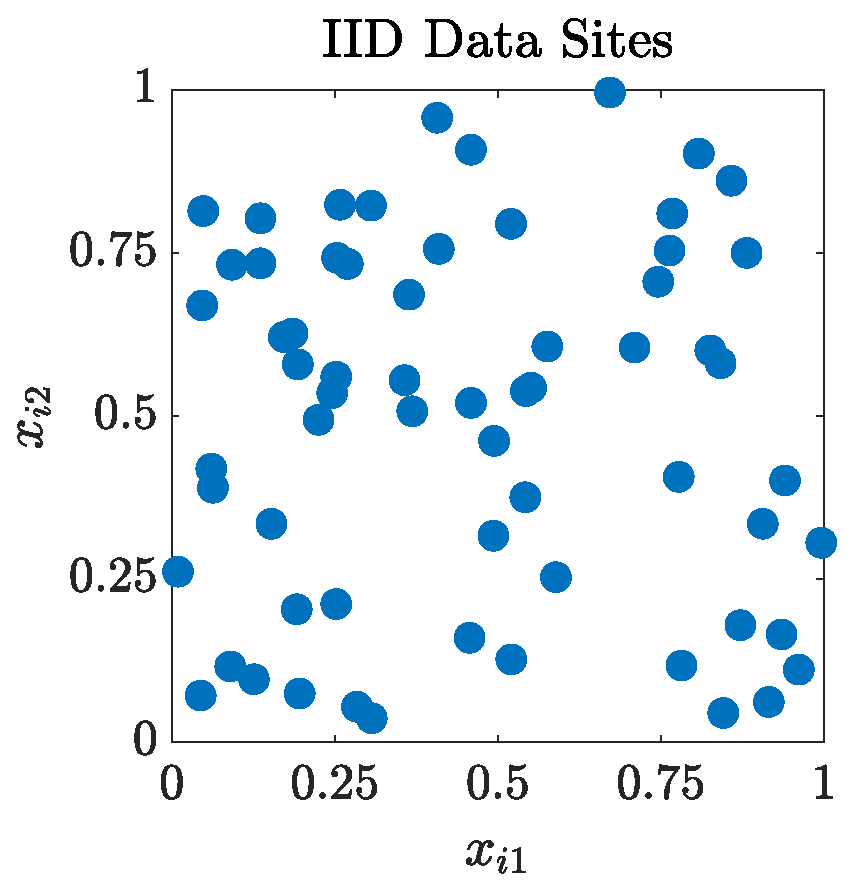
\includegraphics[width = 0.31\textwidth]{ProgramsImages/IIDPoints.eps} \quad
	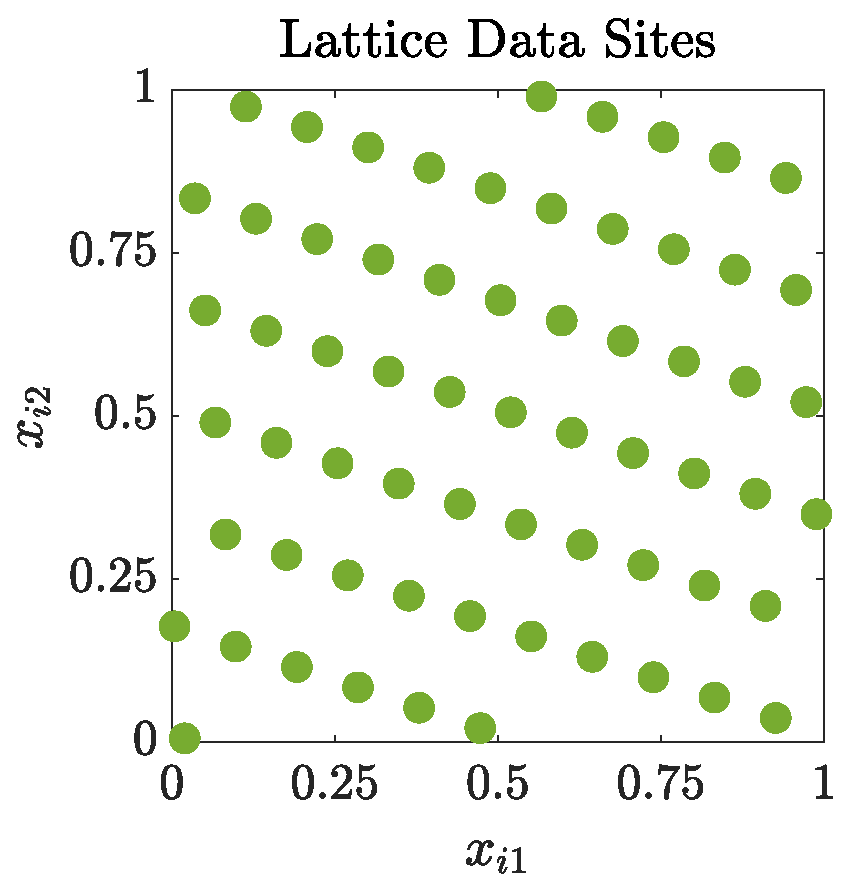
\includegraphics[width = 0.31\textwidth]{ProgramsImages/ShiftedLatticePoints.eps}  \quad
	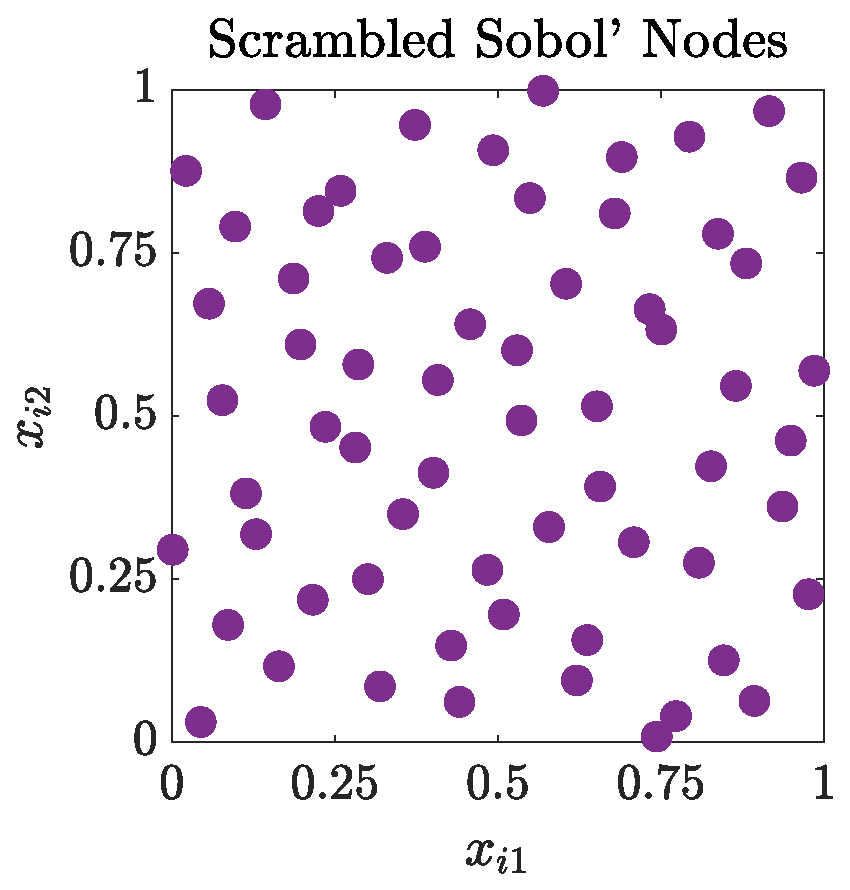
\includegraphics[width = 0.31\textwidth]{ProgramsImages/SSobolPoints.eps} 
	
	\caption{IID data sites contrasted with two families of space filling data sites.\label{PtsFig}}
\end{figure}

The error bounds underlying the adaptive cubatures developed by FJH, LlAJR, DL are based on the Fourier coefficients of the sampled function values on these space-filling designs.  The Fourier  \{complex exponential/Walsh functions\} bases are chosen to match the \{lattices/digital sequences\}  designs, which makes the cubature error bounds possible.  The globally adaptive cubatures increase $n$ by powers of two until the error bounds are no greater than the error tolerance, $\varepsilon$.

The cones, $\calc$, of integrands for which these adaptive cubatures are guaranteed (Key Idea \ref{keyideacone})  are those for which  the Fourier coefficients, $\bigabs{\hf(\bk(\kappa))}$ decay steadily, but not monitonically, in magnitude.  Fig.\ \ref{GoodBadWalshFig} displays a typical function inside $\calc$ and one outside $\calc$. Here $\bk(0), \bk(1), \ldots$ is a natural ordering of the $d$-dimensional wavenumbers.  The function lying outside the cone appears to have high frequency noise. 

\begin{figure}[h]
	\centering
	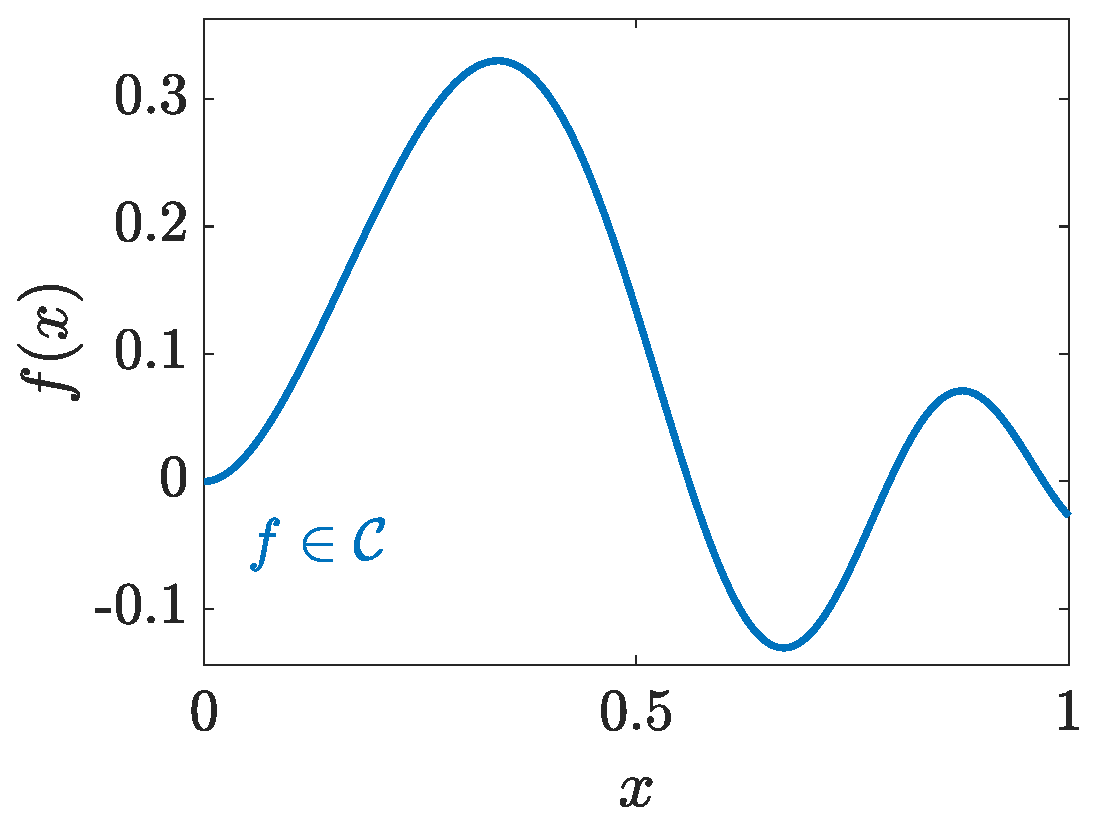
\includegraphics[width = 0.23\textwidth] 
	{ProgramsImages/FunctionWalshFourierCoeffDecay.eps} \ \ 
	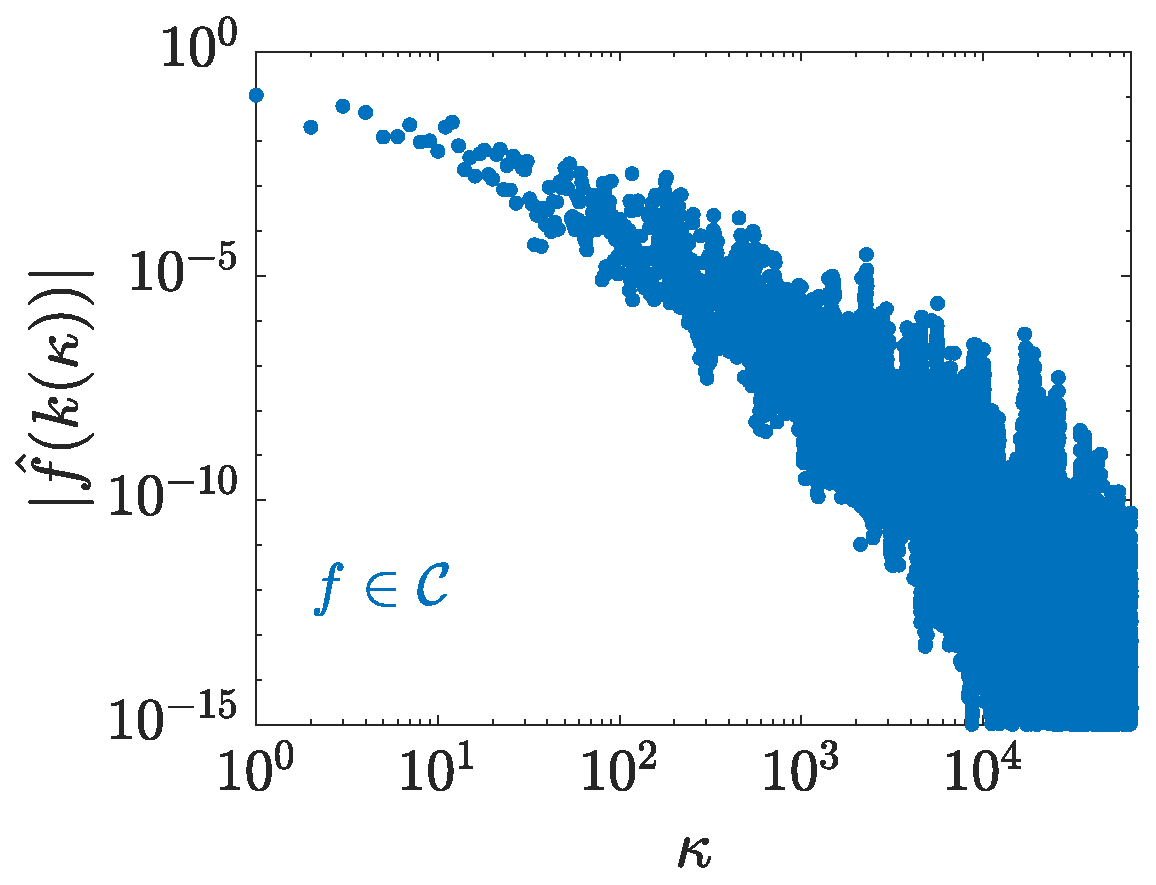
\includegraphics[width = 0.23\textwidth] 
	{ProgramsImages/WalshFourierCoeffDecay128.eps} \ \ 
	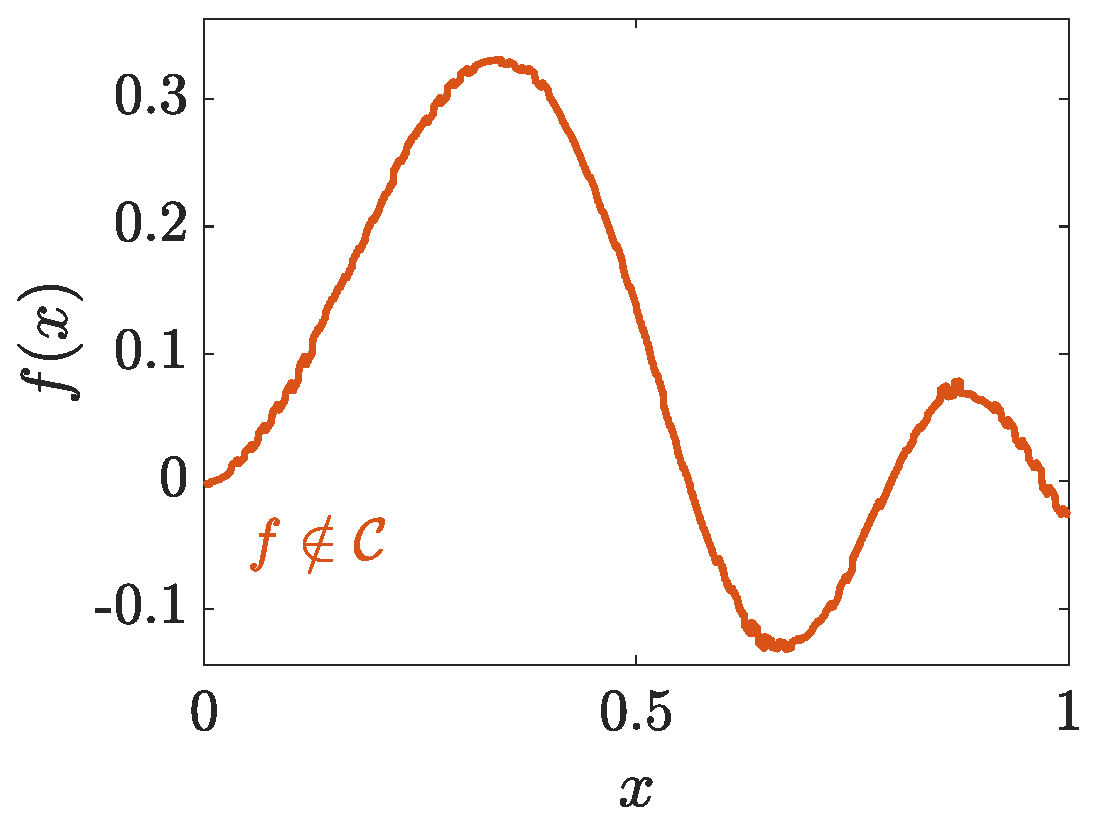
\includegraphics[width = 0.23\textwidth] 
	{ProgramsImages/FilteredFunctionWalshFourierCoeffDecay.eps} \ \ 
	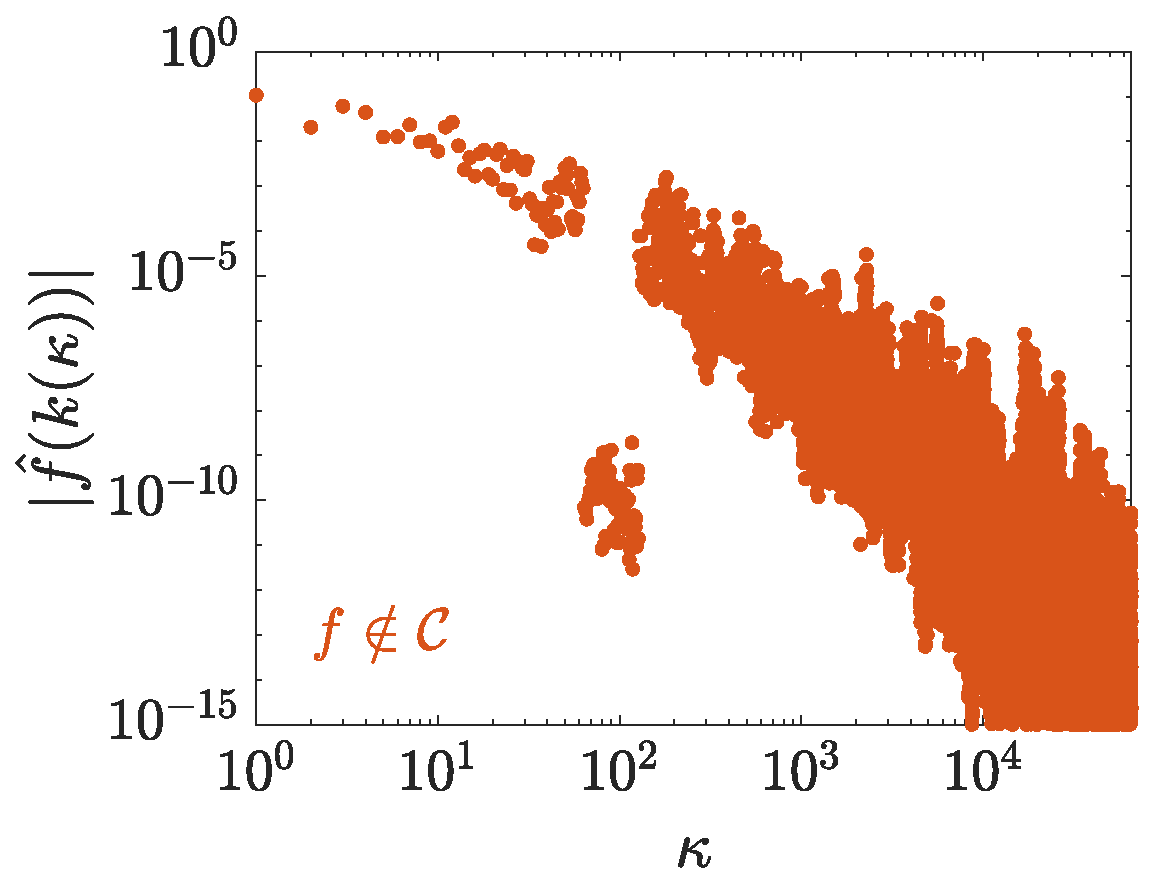
\includegraphics[width = 0.23\textwidth] 
	{ProgramsImages/WalshFourierCoeffDecayFilter.eps}
	\caption{A function inside $\cc$ for which the adaptive algorithms are guaranteed and another function with high frequency noise lying outside $\cc$.
	\label{GoodBadWalshFig}}
\end{figure}

A different approach was taken by FJH and JR, who assumed that the integrand is an instance of a Gaussian process with constant mean $m$, and covariance kernel, $K:[0,1]^d \times [0,1]^d \to \reals$ (Key Idea \ref{keyideaBayesian}).  The same space-filling designs are used as are pictured in Fig.\ \ref{PtsFig}.  A $99\%$ credible interval for the integral is constructed.  The sample size, $n$, is increased until the half-width is no greater than the error tolerance, $\varepsilon$, the algorithm terminates.  The hyper-parameters, $m$ and the parameters defining the covariance kernel, $C$, may be treated by empirical Bayes (maximum likelihood estimation), full Bayes, and/or cross-validation \cite{RatHic19a}. 

The major contribution of FJH and JR is to speed up the computational cost required by this Bayesian cubature.  Bayesian cubature requires operations
involving the Gram matrix $\mK$ defined in \eqref{appxExOne}, and ordinarily these operations  have a cost of
$\Order(n^3)$.  FJH and JR chose covariance kernels, $K$, which matched the space-filling designs and reduced the computational cost to $\Order(n 
\log(n))$, making Bayesian cubature practical.

%%%%%%%%%%%%%%%%%%%%%%%%%%%%%%%%%%%%%%%%%%%%%%%%%%%%%%%%%%%%%%%%%%%%%%%%%%%%%%%%%%%
\subsubsection{Multivariate Function Approximation} \label{sec:PrevFunAppx}
%%%%%%%%%%%%%%%%%%%%%%%%%%%%%%%%%%%%%%%%%%%%%%%%%%%%%%%%%%%%%%%%%%%%%%%%%%%%%%%%%%%

FJH, YD, and LlAJR and collaborators investigated the function approximation problems that resemble the setting in Sect.\ \ref{ex:multi}, but more generally allowing the basis $\{u_{\bk}\}_{\bk \in \bbK}$ to be general multivariate polynomials \cite{DinHic20a,DinEtal20a}.  Three different definitions of cones of functions were defined, all describing a reasonable behavior of the series coefficients.  Adaptive function approximation algorithms were constructed for these three cones shown to be essentially optimal.  The shortcoming of this research is that the algorithms use series coefficients rather than function values. 


%%%%%%%%%%%%%%%%%%%%%%%%%%%%%%%%%%%%%%%%%%%%%%%%%%%%%%%%%%%%%%%%%%%%%%%%%%%%%%%%%%%
\subsection{Broader Impacts from Previous NSF Funding} \label{prevBIsect}
%%%%%%%%%%%%%%%%%%%%%%%%%%%%%%%%%%%%%%%%%%%%%%%%%%%%%%%%%%%%%%%%%%%%%%%%%%%%%%%%%%%

\emph{Publications, Conference Participation, Conference Organization, and Leadership.} Publications by GEF, FJH,  SCTC, students, and collaborators are listed at the beginning of this section.  We have spoken at many applied mathematics, statistics, 
and computational science conferences and given colloquium/seminar talks to mathematics and 
statistics departments.  FJH co-organized the 
\href{http://cos.iit.edu/2016-spring-research-conference/}{2016 Spring Research 
Conference}, a long-running annual industrial statistics conference.   FJH gave an invited tutorial
at \href{http://mcqmc2016.stanford.edu}{MCQMC 2016} 
\cite{Hic17a}, a biennial conference for which he serves on the steering committee.  FJH 
was a program leader for the SAMSI 2017--18 
\href{https://www.samsi.info/programs-and-activities/year-long-research-programs/2017-18-program-quasi-monte-carlo-high-dimensional-sampling-methods-applied-mathematics-qmc/
}{Quasi-Monte Carlo (QMC) Program (\hypertarget{SAMSIlink}{SAMSI-QMC})}.   FJH received the 2016 Joseph F.\ Traub Prize for Achievement in Information-Based Complexity. In recognition of his research leadership, FJH was appointed the director of Illinois Tech's new Center for Interdisciplinary 
Scientific Computation in 2017.  In 2018, FJH was appointed Vice Provost for Research.

	
\emph{\GAIL Software.} The results of this research have been implemented in 
\GAIL, our open source \MATLAB library hosted on
\href{http://gailgithub.github.io/GAIL_Dev/} {Github}. This software 
has been implemented with input parsing, input validation, unit tests, inline documentation, and 
demonstrations.  \GAIL makes it easier for practitioners to try our new adaptive algorithms.  SCTC has been key in this effort.  \GAIL has been used in the yearly graduate course in Monte Carlo methods taught by FJH and YD.  
%With the help of students, we are starting to port GAIL to Python and \Rlang.

\emph{Boosting the STEM Workforce.} GEF, FJH, and SCTC mentored a number of 
research students associated with this project.  Female students mentored include YD, LJ, JL, XT, and Xiaoyang Zhao (MS 2017).   GEF, FJH,  and SCTC have mentored many undergraduate students including more than a dozen 
Brazilian Science Mobility Program students in the summers of 2015 and 2016, plus eight other students (two female) from Illinois Tech, Biola U, U Minnesota, Macalester U, NUS, Colorado School of Mines.  All but one have enrolled in graduate programs.   As part of our team, all of
these students have learned how to conduct theoretical and/or practical computational mathematics research.

%%%%%%%%%%%%%%%%%%%%%%%%%%%%%%%%%%%%%%%%%%%%%%%%%%%%%%%%%%%%%%%%%%%%%%%%%%%%%%%%%%%
\section{Intellectual Merit of the Proposed Research} \label{sec:Proposed}
%%%%%%%%%%%%%%%%%%%%%%%%%%%%%%%%%%%%%%%%%%%%%%%%%%%%%%%%%%%%%%%%%%%%%%%%%%%%%%%%%%%

%%%%%%%%%%%%%%%%%%%%%%%%%%%%%%%%%%%%%%%%%%%%%%%%%%%%%%%%%%%%%%%%%%%%%%%%%%%%%%%%%%%%
\subsection{Shortcomings of Existing Adaptive Sampling Schemes} \label{sec:shortExist}
%%%%%%%%%%%%%%%%%%%%%%%%%%%%%%%%%%%%%%%%%%%%%%%%%%%%%%%%%%%%%%%%%%%%%%%%%%%%%%%%%%%

%%%%%%%%%%%%%%%%%%%%%%%%%%%%%%%%%%%%%%%%%%%%%%%%%%%%%%%%%%%%%%%%%%%%%%%%%%%%%%%%%%%
\subsection{Reproducing/Covariance Kernels Inferred from Data} \label{sec:kerinferdata}
%%%%%%%%%%%%%%%%%%%%%%%%%%%%%%%%%%%%%%%%%%%%%%%%%%%%%%%%%%%%%%%%%%%%%%%%%%%%%%%%%%%
Key Idea \ref{keyideafunction} stresses the importance of having the choice of the next data site depend on function data.  The function, $f$, that we intend to approximate belongs to an infinite number of function spaces or cones within those function spaces.  Our adaptive sampling scheme should help identify a function space for which $f$ is typical, not an unusual.  Returning to the illustrative example in Sect.\ \ref{sec:UniEx}, the lack of fit of our approximation on the left and our poor choice of the next data site based on the approximation error bound is due to the fact that the form of our reproducing kernel in \eqref{MatKer} and/or our choice of $\theta$ was inadequate.

The value of $\theta$ can be inferred using an empirical Bayes perspective (Key Idea \ref{keyideaBayesian}), which leads to the following optimization problem \cite{Hic17a}: 
\begin{equation}
    \theta_{\textup{EB}} = \argmin_\theta \left[\frac 1n \log \bigl( \det(\mK_\theta) \bigr) + \log \bigl ( \by_{1:n}^T \mK_\theta^{-1} \by_{1:n} \bigr)\right].
\end{equation}
For the example in Sect.\ \ref{sec:UniEx}, $\theta_{\textup{EB}} = 20$, and it is 

\begin{figure}
    \centering
    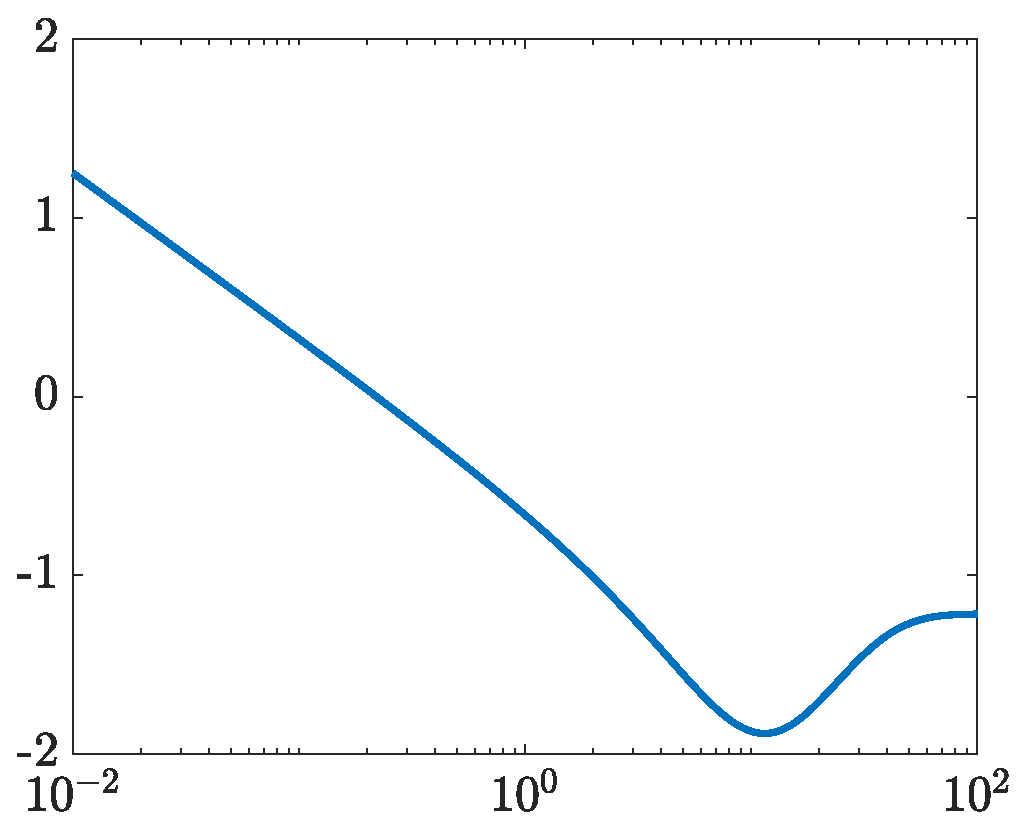
\includegraphics[width = 7cm]{ProgramsImages/fandDataAndOptAppx.eps} \qquad \qquad
    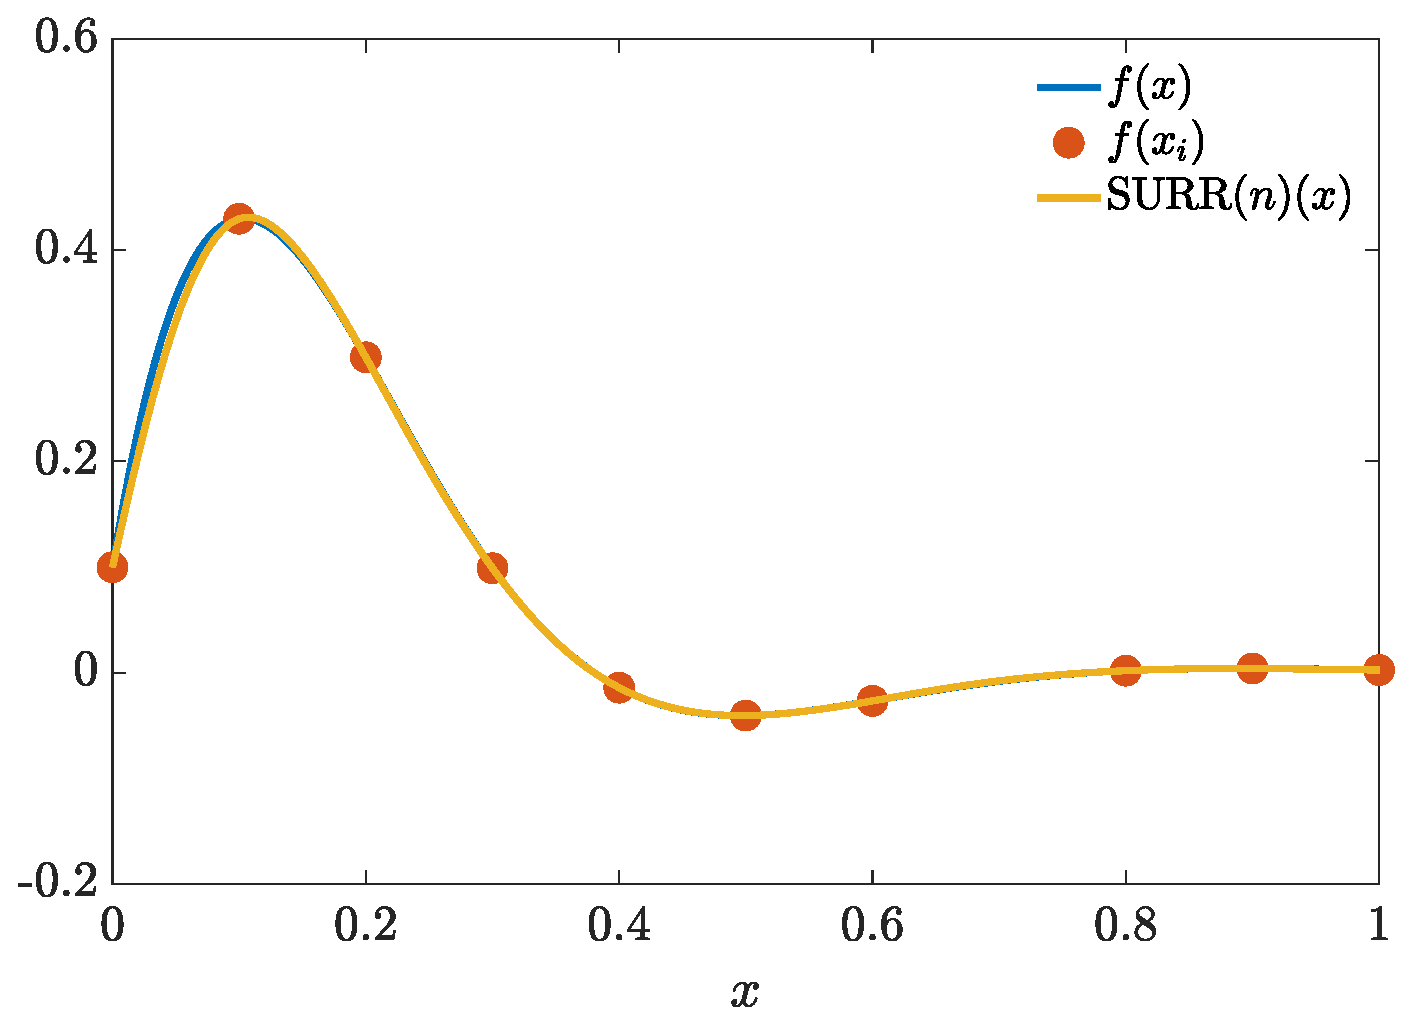
\includegraphics[width = 7cm]{ProgramsImages/fandDataAndOptyAppx.eps}
    \caption{Caption}
    \label{fig:my_label}
\end{figure}




%%%%%%%%%%%%%%%%%%%%%%%%%%%%%%%%%%%%%%%%%%%%%%%%%%%%%%%%%%%%%%%%%%%%%%%%%%%%%%%%%%%
\subsection{Detrending} \label{sec:detrending}
%%%%%%%%%%%%%%%%%%%%%%%%%%%%%%%%%%%%%%%%%%%%%%%%%%%%%%%%%%%%%%%%%%%%%%%%%%%%%%%%%%%

%%%%%%%%%%%%%%%%%%%%%%%%%%%%%%%%%%%%%%%%%%%%%%%%%%%%%%%%%%%%%%%%%%%%%%%%%%%%%%%%%%%
\subsection{Selecting Importanct Coordinates} \label{sec:seletCoord}
%%%%%%%%%%%%%%%%%%%%%%%%%%%%%%%%%%%%%%%%%%%%%%%%%%%%%%%%%%%%%%%%%%%%%%%%%%%%%%%%%%%

%%%%%%%%%%%%%%%%%%%%%%%%%%%%%%%%%%%%%%%%%%%%%%%%%%%%
\subsection{Test Bed of Practical Problems} \label{sec:TestBed}
%%%%%%%%%%%%%%%%%%%%%%%%%%%%%%%%%%%%%%%%%%%%%%%%%%%%



%%%%%%%%%%%%%%%%%%%%%%%%%%%%%%%%%%%%%%%%%%%%%%%%%%%%
\section{Broader Impacts of the Proposed Research}\label{SectBroad}
%%%%%%%%%%%%%%%%%%%%%%%%%%%%%%%%%%%%%%%%%%%%%%%%%%%%
\FJHNote{This is copied from my old proposal.  Must be revised.}


%%%%%%%%%%%%%%%%%%%%%%%%%%%%%%%%%%%%%%%%%%%%%%%%%%%%
\subsection{Contributions to Training, Mentoring and Other Human Resource Developments}
%%%%%%%%%%%%%%%%%%%%%%%%%%%%%%%%%%%%%%%%%%%%%%%%%%%%
FJH leads a weekly research group meeting comprised of long-term and short-term student 
collaborators, visitors, the curious, and special guests.  Ongoing work in early or polished stages is shared.  Papers of other authors are presented.  Mentoring takes place during these meetings as well as individually.

\emph{Providing Research Experiences for Undergraduate and High School Students.} Students 
should be introduced to research before graduate school so that they can learn how to 
discover the unknown, something that is not necessarily taught in the classroom. We request funds 
to 
support two summer undergraduate students per year.  Our small summer research program has established some visibility 
and is prompting inquiries from prospective participants well before we 
even announce our latest 
offerings. As in the past, we expect the NSF funds will serve as a catalyst for funds to 
support additional summer students. In choosing summer students we will make a deliberate effort to 
build 
a diverse research environment by targeting female and underrepresented minority students as well 
as students from less research-focused institutions (see Sect.~\ref{prevBIsect}). We will also 
welcome well-prepared high school students to join our research group.

\emph{Preparing Students for Academic Careers.} Mentoring is a multi-faceted and 
potentially long-term process continuing even after the mentee has moved on from Illinois Tech.  
Our PhD students gain experience both research and mentoring the younger students in our 
research group.  We 
continue contact with many of our former students.  In particular we continue to 
collaborate with YD and Yiou Li (female).  We will continue to help our students prepare for 
academic careers and continue mentoring them after they leave Illinois Tech.

\emph{Preparing Students for Industry Careers.}
We also help current students land 
competitive jobs in the business world. Our training in the areas of computation and software 
development gives our students the needed edge in comparison to other mathematics 
graduates. For example, LlAJR and XZ are working in the financial services industry and  LJ is 
working in marketing analytics.  All of them are developing and testing quantitatively sophisticated 
and computationally intensive models.  LlAJR and LJ continue to collaborate with us on research.

\emph{Supervising Visitors.}
Both FJH and SCTC have strong connections to East Asia.  We have hosted several long-term 
self-funded visitors in the past and plan to do so in the future.

\emph{Giving Tutorials and Invited Lectures.}
We will continue providing lectures to students at various stages in their careers, ranging from high
school to graduate school. These encourage students to enter STEM and encourage STEM students 
to engage in research in general, and this research area in particular.


%%%%%%%%%%%%%%%%%%%%%%%%%%%%%%%%%%%%%%%%%%%%%%%%%%%%
\subsection{Contributions to Resources in Research, Education and the Broader Society} 
\label{BroaderTwoSec}
%%%%%%%%%%%%%%%%%%%%%%%%%%%%%%%%%%%%%%%%%%%%%%%%%%%%

The proposed research straddles mathematics, statistics, theoretical computer science, and 
application areas.  The two PIs have complementary strengths that facilitate this interdisciplinary research.  FJH 
has expertise in \QMC methods, kernel-based methods, information-based complexity 
theory, tractability, and experimental design. SCTC has expertise in computer science and applications.  Our 
expertise provides both an obligation and an opportunity to interact with a number of diverse 
communities. We envision the following contributions:

\emph{Disseminating Research}
The research supported by this grant will result in publications in peer-reviewed journals in applied
mathematics, computer science, statistics, and science/engineering. These 
journals will include both those that emphasize theory and those that emphasize applications.

\emph{Promoting Cones.} The idea of guaranteed, adaptive algorithms via cones of reasonable input 
functions has broad potential application.  We will continue to promote this idea among numerical analysts 
who 
develop new algorithms and analyze their computational costs, as well as among information-based 
complexity theorists who analyze the lower bounds on the complexity of numerical problems.  The recent work by Kunsch, Novak, and Rudolf \cite{KunEtal19a} shows that the idea of cones is catching on.

\emph{Bridging Applied Mathematics and Statistics.}
This project touches on topics that are of interest to the statistics community: kriging, Monte Carlo methods, probabilistic numerics, and design of experiments.  We have and will continue to engage the statistics community 
by speaking a their conferences and departmental colloquia.

\emph{Organizing and Presenting at Conferences.}
We and our students involved in this project will present our results at a variety of conferences and workshops.  These include: (i) specialized meetings focusing on approximation theory, complexity, 
experimental design, Monte Carlo methods, and probabilistic numerics; (ii) the national meetings of AMS, SIAM, and the 
statistical societies; and (iii) conferences devoted to application areas.  We are frequently invited to 
speak at such conferences, which will give our results a prominent hearing. We will also continue to 
organize specialized conferences or minisymposia within larger conferences.

\emph{Writing Survey Papers.}
FJH and SCTC will continue their practice of writing tutorial, survey, and encyclopedia articles.  These will make our findings accessible to a wider audience.

\iffalse
\emph{Refreshing Course Syllabi.}
MATH 565 (Monte Carlo Methods in Finance), taught every fall by FJH, has incorporated our new
results on guaranteed (quasi-)Monte Carlo multivariate integration. In the future it will include our 
new results on our guaranteed MLM and MDM (see Sect.\ \ref{SectMultiProb}).

As noted in Sect.\ \ref{TrapIllSect}, current texts propagate poor practices for 
adaptive quadrature.  We will urge numerical analysis textbook authors and educators to change the 
way that error estimation is taught based on our recent and proposed work.  These ideas will also 
enter our more traditional numerical analysis courses such as MATH 350 (Intro to Computational 
Math).  SCTC and FJH will continue to develop MATH 573 (Reliable Mathematical Software) as a 
valuable course for our own students and an example that we wish to propagate to other 
universities.
\fi

\emph{Creating Software and Collaborating with Software Developers.}
As the complexity of large scale numerical computations increase rapidly, mundane operations such as integration and function approximation are taken for granted. We must construct reliable adaptive algorithms for these problems so that there are no unwelcome surprises for the practitioner when she takes them for granted.

We will continue to develop \GAIL \citep{ChoEtal17b} (now up to version 2.2).  The \GAIL software 
will serve the wider community that relies on numerical approximation and integration algorithms.  It will 
also demonstrate how adaptive algorithms ought to be implemented, which we hope will inspire and 
inform those working on adaptive algorithms for other mathematical problems.  We will involve 
students in porting \GAIL to other platforms, such as Python, \Rlang, and \Julia.  

In the summer of 2018, we began engaging with other \QMC research groups about combining our software efforts.  These included the groups of Mike Giles (Oxford, Multi-Level Monte Carlo),  Frances Kuo (UNSW, \QMC generators, PDEs with random coefficients),  Dirk Nuyens (KU Leuven, \QMC generators, PDEs with random coefficients), and Christoph Schwab (ETH-Zurich, PDEs with random coefficients).  All of these groups have significant software development efforts, but our software libraries are not compatible with one another.  We have begun discussing a common framework for a shared community quasi-Monte Carlo software library, \QMCSoft.  If all groups would write their software to the specifications of this framework, then improvements and additions would immediately work with the other parts of the library.

We will collaborate with these other research groups to move our software to this common framework.  Given the difficulty in agreeing upon one language, this may be a multi-language effort.  We will seek resources outside this proposal to support this effort.  As the \QMC community embraces \QMCSoft, we expect our core of contributors to grow.  Scholars who develop new \QMC algorithms or use \QMC in applications will be encouraged to add them to \QMCSoft.  

We expect our new algorithms to be incorporated into widely used numerical packages, as was done for our algorithm in \cite{HonHic00a} by \MATLAB and \NAG.  We have already and will continue 
to discuss with software developers about good practices for adaptive algorithms.


\emph{New Applications of \QMC.}
The application of \QMC has focused on a few areas, such as financial modeling and computer 
graphics, but there is potential for much wider application.  LlAJR has collaborated with Fermilab implementing \QMC algorithms, and we plan to continue.    New applications of \QMC are arising from \SAMSIQMC that we plan to pursue.  KZ is exploring how to use adaptive \QMC to more efficiently perform Bayesian inference.


\newpage
\clearpage
%\pagenumbering{arabic}
\setcounter{page}{1}

\bibliographystyle{spbasic.bst}


{\renewcommand\addcontentsline[3]{} 
\renewcommand{\refname}{{\Large\textbf{References Cited}}}                   %%
\renewcommand{\bibliofont}{\normalsize}

\bibliography{FJH23,FJHown23}}
\end{document}


